\documentclass{slide}

\usepackage{changepage}
% \usepackage{pgfpages}
% \setbeameroption{show notes on second screen}

\title{Architectural Skills}
\subtitle{CSSE6400}
\author{Richard Thomas}
\date{\week{13}}

\begin{document}

\maketitle

\point[Quote]{Architecture is the stuff you can't Google.\\
 ~~~~~ -- Mark Richards \cite{richards2020fundamentals}}

\point[Quote]{There are no right or wrong answers in architecture---only trade-offs.\\
 ~~~~~ -- Neal Ford \cite{richards2020fundamentals}}

\point[Architectural Design]{Architects use knowledge and experience to analyse trade-offs to design architectures appropriate to the system context.}

\begin{frame}{Developers -- Technical Depth \cite{richards2020fundamentals}}
    \centering
    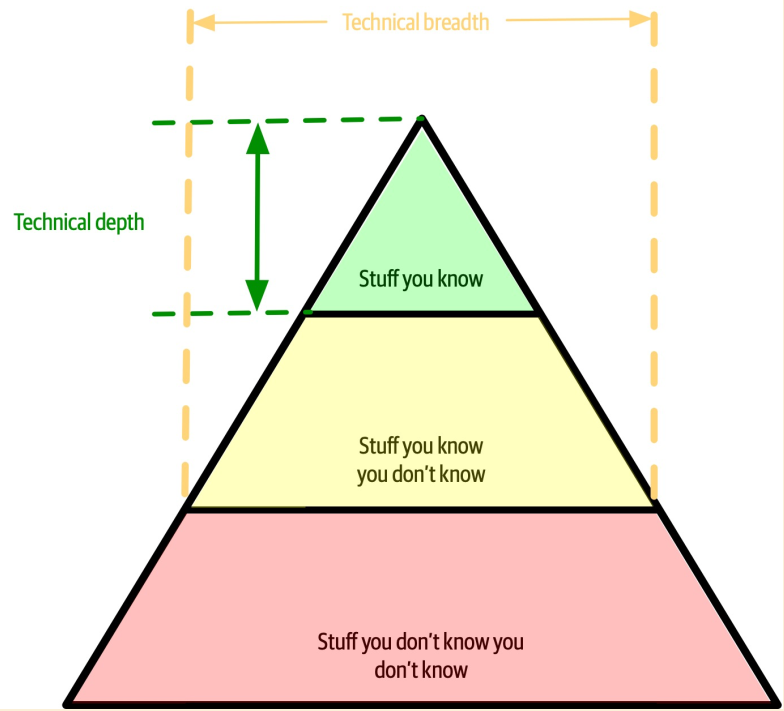
\includegraphics[trim=1 1 1 1,clip,height=0.92\textheight]{images/depth-breadth-pyramid-1.png}
\end{frame}

\begin{frame}{Architects -- Technical Breadth \cite{richards2020fundamentals}}
    \centering
    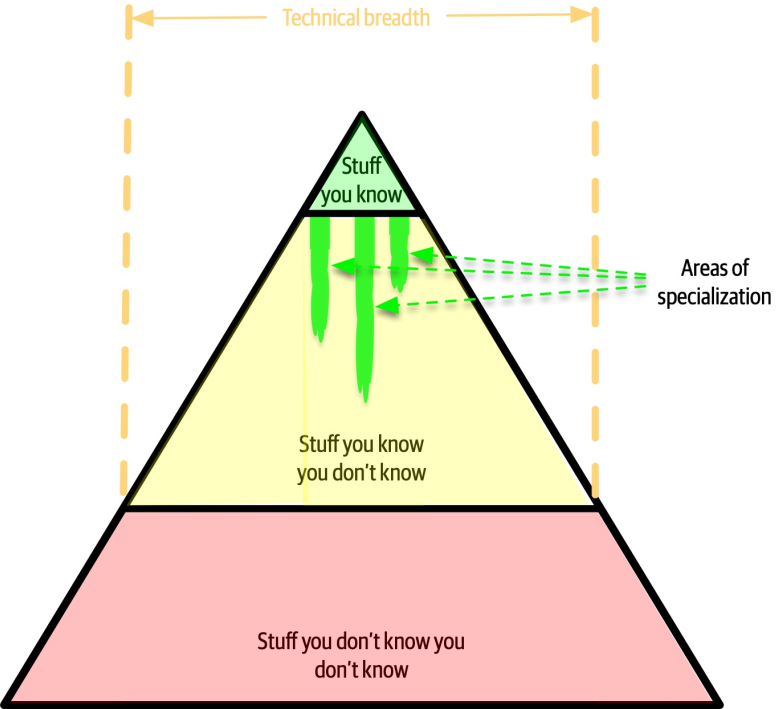
\includegraphics[trim=1 1 1 1,clip,height=0.92\textheight]{images/depth-breadth-pyramid-2.png}
\end{frame}
\note[itemize]{
    \item Architects need greater technical breadth than depth.
    \item Breadth allows better consideration of trade-offs.
    \item Avoid trying to become an expert across many areas -- you'll fail.
    \item Don't stop learning -- increase your breadth -- don't let your knowledge become stale.
}

\questionanswer{What are the benefits of a monolith architecture?}{
    \begin{itemize}[<+(1)->]
        \item Simple deployment
        \item Simple communication between modules
        \item Simple system testing \& debugging
    \end{itemize}
}

\questionanswer{Why do monoliths have a bad name?}{
    \begin{itemize}[<+(1)->]
        \item Many legacy system nightmares were monoliths
        \item Easy to defeat modularity
        \item Cannot scale components of system
        \item Monolith databases scale poorly
    \end{itemize}
}

\questionanswer{What can be done if a monolith architecture is no longer suitable?}{
    \begin{itemize}[<+(1)->]
        \item Greenfields replacement
        \item Migrate to another architecture
    \end{itemize}
}
\note[itemize]{
    \item Replacement: Can choose any suitable architecture. Risky, as you're developing a new system and maintaining existing.
    \item Migration: Adaptive maintenance, changing architecture slowly. Some limitation on choice of architecture, but most sophisticated architecture can be used.
}

\questionanswer{How do I migrate a monolith to a new architecture?}{Decompose the monolith into services.}
\note{Implies a service-based or microservices architecture.}

\begin{frame}{Strangler Fig Pattern}
    \vspace{1pt}
    \begin{columns}
    \column{0.65\textwidth}
      {\LARGE
        \begin{itemize}
            \item Develop API for application's UI
            \vspace{1mm}
            \item Proxy intercepts API calls
            \begin{itemize}
                \Large\item Proxy directs calls to application or new services
            \end{itemize}
            \vspace{1mm}
            \item Implement a service
            \begin{itemize}
                \Large\item Redirect calls to service
            \end{itemize}
            \item Progressively replace monolith
            \item Shadow \& Blue-Green Deployment
        \end{itemize}
      }
    \column{0.35\textwidth}
        \centering
        
\includegraphics[height=0.9\textheight]{images/strangler-fig.jpg}
    \end{columns}
\end{frame}
\note[itemize]{
    \item May already have an API if the UI is a web or mobile app.
    \item Initially deploy proxy and new interface into production, with only existing monolith. Test it works as expected.
    \item Use shadow deployment to test service with application, before making available to end users.
}

\begin{frame}{Monolith Deployment}
    \begin{adjustwidth}{-12mm}{-12mm}
        \centering
        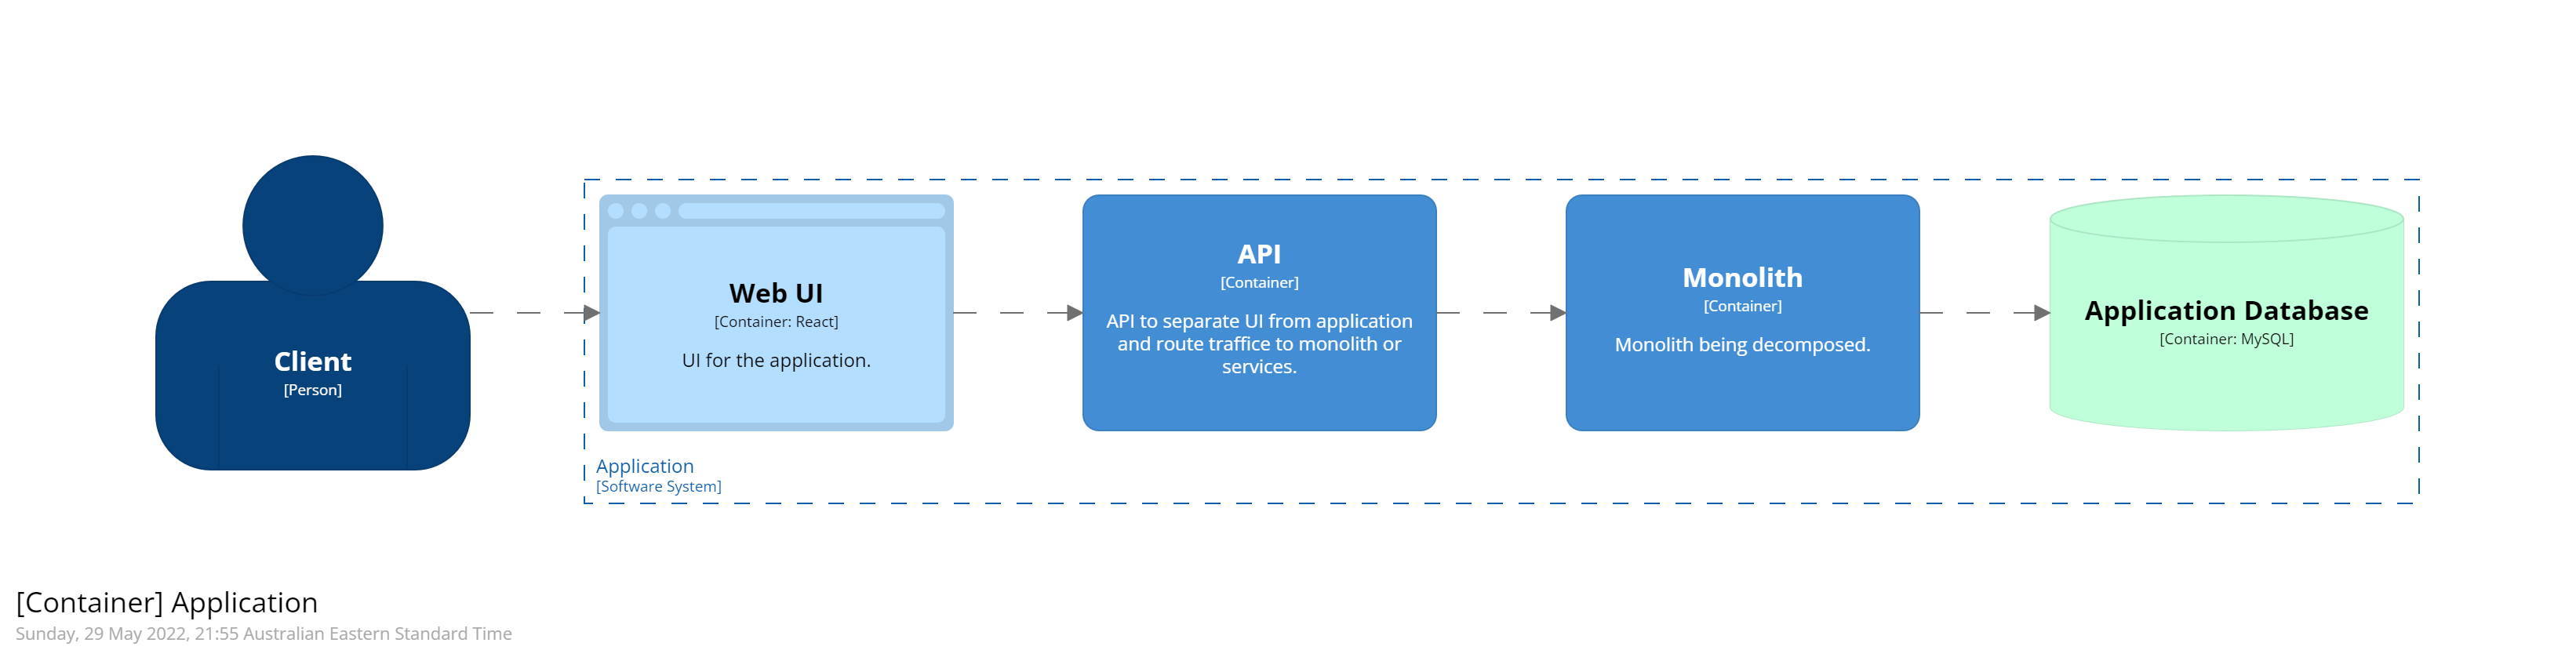
\includegraphics[trim=195 195 195 195,clip,width=0.97\paperwidth]{diagrams/decompose1.png}
    \end{adjustwidth}
\end{frame}

\begin{frame}{Monolith Decompose: Step 1}
    \begin{adjustwidth}{-12mm}{-12mm}
        \centering
        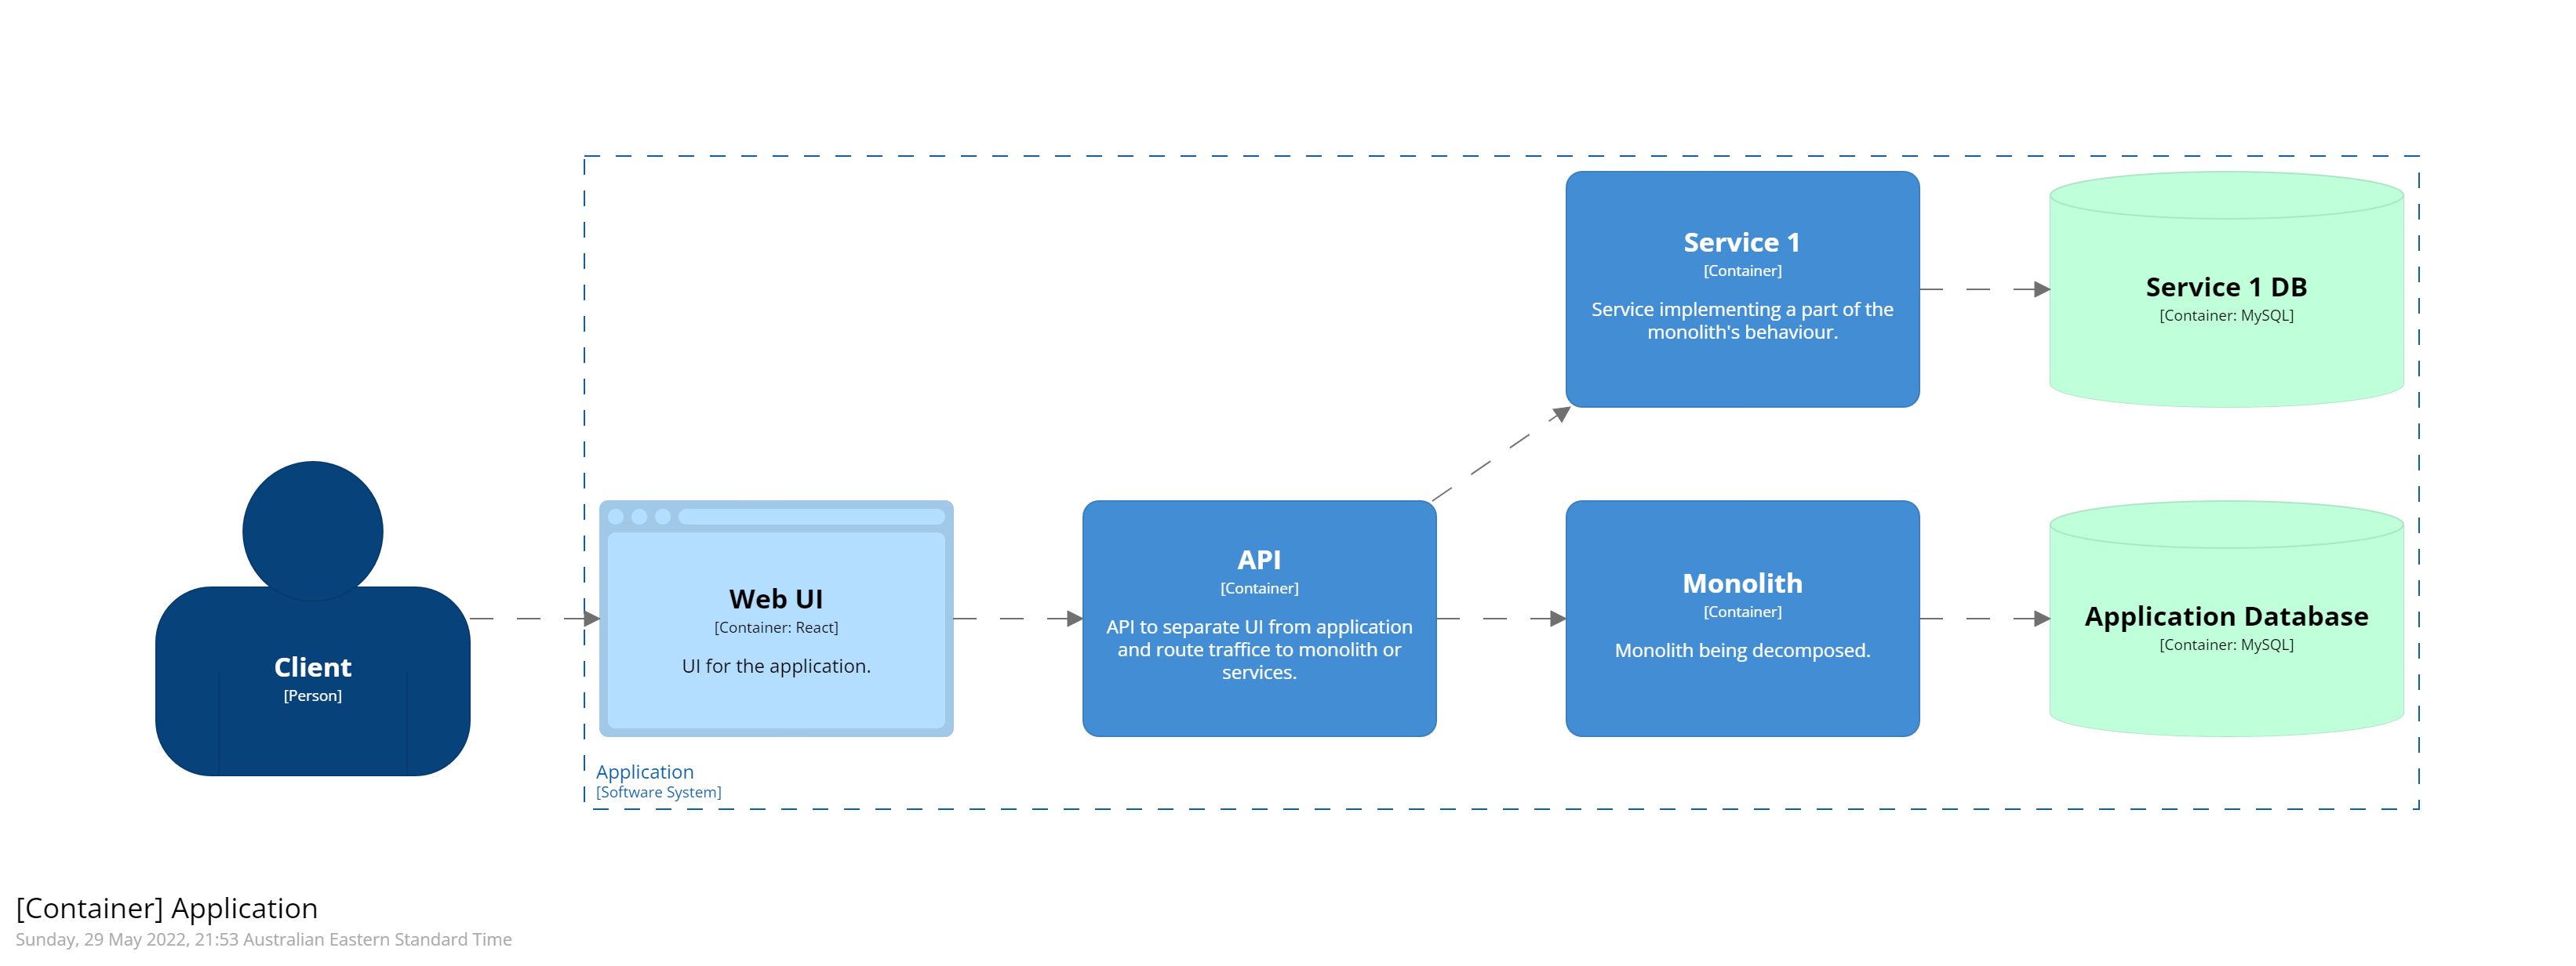
\includegraphics[trim=195 195 195 195,clip,width=0.97\paperwidth]{diagrams/decompose2.png}
    \end{adjustwidth}
\end{frame}

\begin{frame}{Monolith Decompose: Step 2}
    \begin{adjustwidth}{-12mm}{-12mm}
        \centering
        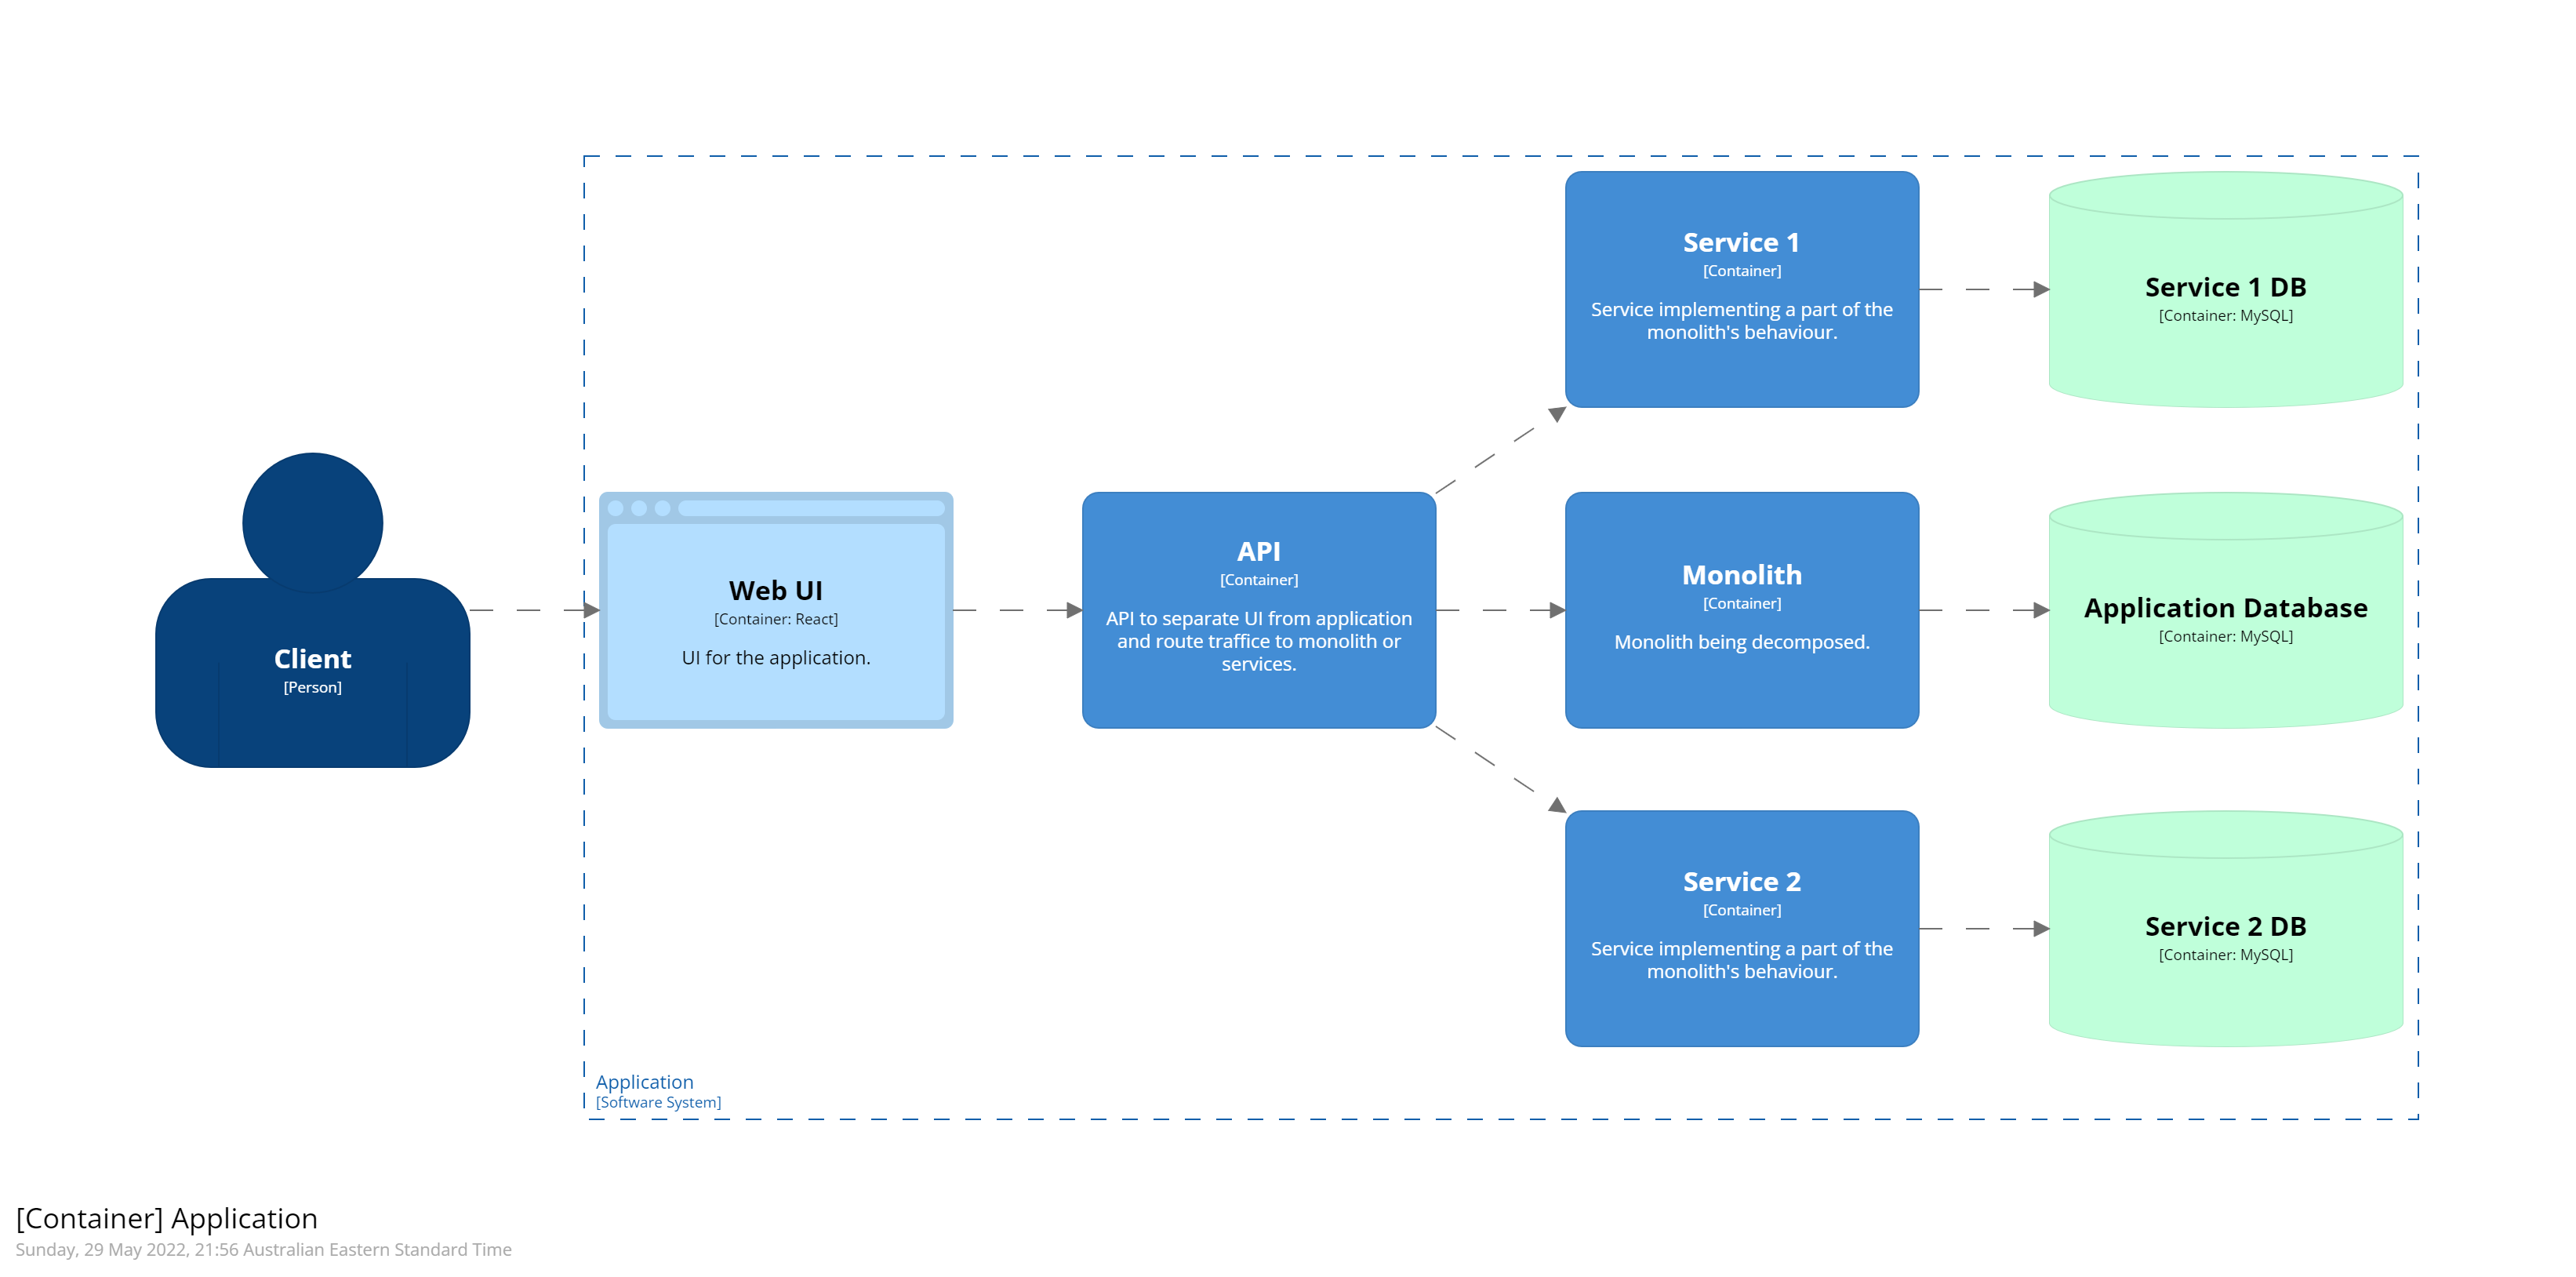
\includegraphics[trim=195 195 195 195,clip,width=0.97\paperwidth]{diagrams/decompose3.png}
    \end{adjustwidth}
\end{frame}

\begin{frame}{Decomposition Process}
\vspace{1pt}
{\huge
\begin{itemize}
    \item Identify bounded-contexts
    \vspace{1mm}
    \item Simple first service
    \begin{itemize}
        \LARGE\item e.g. Authentication
    \end{itemize}
    \vspace{1mm}
    \item Minimise dependency from services to monolith
    \begin{itemize}
        \LARGE\item Monolith may use services
    \end{itemize}
\end{itemize}
}
\end{frame}
\note[itemize]{
    \item Use first service (or first few) to validate approach and deployment infrastructure.
    \item Minimise changes required in monolith.
}

\begin{frame}{Decomposition Process}
\vspace{1pt}
{\huge
\begin{itemize}
    \item Reduce coupling between bounded- contexts
    \vspace{2mm}
    \begin{itemize}
        \LARGE\item e.g. Customer account management
        \begin{itemize}
            \Large\item Profile, Wish List, Payment Preferences -- separate services
        \end{itemize}
    \end{itemize}
    \vspace{2mm}
    \item Decouple vertically
    \vspace{1mm}
    \begin{itemize}
        \LARGE\item Service delivers entire bounded-context
        \begin{itemize}
            \Large\item Data is decoupled from monolith
        \end{itemize}
    \end{itemize}
\end{itemize}
}
\end{frame}
\note[itemize]{
    \item Account management may be tightly coupled in monolith. Separate each aspect (context), one at a time.
    \item Do not focus only on UI or internal components, service needs to implement all parts of the business process.
    \item Data management needs to be decentralised.
}

\begin{frame}{Decomposition Process}
\vspace{1pt}
{\huge
\begin{itemize}
    \item Focus on pain points
    \begin{itemize}
        \LARGE\item Bottlenecks
        \LARGE\item Frequently changing behaviour
    \end{itemize}
    \vspace{1mm}
    \item Rewrite, don't reuse
    \begin{itemize}
        \LARGE\item Redesign for new infrastructure
        \vspace{1mm}
        \LARGE\item Reuse complex logic
        \begin{itemize}
            \Large\item e.g. Discounts based on customer loyalty and behaviour, bundle offers, \dots
        \end{itemize}
    \end{itemize}
\end{itemize}
}
\end{frame}
\note[itemize]{
    \item Extract services that deliver highest value.
    \item What contexts may need to scale more than others?
    \item What contexts change more frequently and benefit from separate deployment?
    \item Services deliver capabilities provided by monolith.
    \item Most often it is better to rewrite the capability to take advantage of new infrastructure.
    \item Only reuse code that has complex logic that will be difficult to duplicate and test fully.
}

\begin{frame}{Atomic Decomposition}
\vspace{1pt}
{\huge
\begin{itemize}
    \item Refactor monolith
    \vspace{2mm}
    \begin{itemize}
        \LARGE\item Use service to deliver application functionality
        \begin{itemize}
            \Large\item Monolith may need to invoke service
        \end{itemize}
        \LARGE\item Remove service logic from monolith
    \end{itemize}
\end{itemize}
}
\end{frame}
\note[itemize]{
    \item Atomic replacement of monolith behaviour by service's behaviour.
    \item Don't deploy production code with service behaviour left in monolith.
            Leads to a maintenance nightmare determining where behaviour is used, or it may be used in both the monolith and service.
}

\point[Stepwise Decomposition]{Replace application functionality one service at a time.}

\definition{Macroservice}{Separate service, but may span more than one domain or share a database with the monolith or other services.}
\note[itemize]{
    \item Similar scalability and deployment issues to a monolith, but grouped by clusters of macroservices if they share a database.
    \item Interim step to build microservices.
}

\definition{Nanoservice}{Service that depends on other services and cannot be deployed independently -- its context is too small.}
\note[itemize]{
    \item Anti-pattern where services are too fine grained and need to be coupled to deliver business processes.
    \item Some use the term ``nanoservice'' to refer to independently deployable functions, similar to serverless architecture.
}

\definition{Conway's Law}
{Organisations design systems whose structure is inevitably a copy of the organisation's communication structure \cite{conways-law} \cite{maccormack2012}.}
\note[itemize]{
    \item First citation is original article.
    \item Second citation is one of several about MIT and Harvard research into the phenomenon, calling it the ``mirroring hypothesis''.
    \item Elaborate on this point and Coplien's research into organisational sociology.
}

\point[Conway's Law Consequences]{
\begin{itemize}
    \item Business Process Management
    \item Microservices to reflect organisation structure
    \item Teams formed around services
\end{itemize}
}
\note[itemize]{
    \item BPM: Redesign organisation structure to reflect system you want.
    \item Microservices: Design system to reflect your organisation.
    \item Elaborate on benefits of both approaches.
    \item Comment on benefits of small focussed teams.
}

\point[Conway's Law Consequences]{Team insularity -- more loyal to team than organisation.}
\note[itemize]{
    \item Amazon example from week 11, negotiation difficulties with other teams.
    \item Need to ensure inter-team cooperation.
    \item Possibly move people between teams.
    \item Cloud platforms, and microservices, also support this and with larger teams.
    \item Intra-team communication becomes more difficult with large teams.
}

\begin{frame}{Conway's Law Issues}
\vspace{1pt}
{\huge
\begin{itemize}
    \item Cross-cutting concerns
    \begin{itemize}
        \LARGE\item e.g. Security
    \end{itemize}
    \item Organisation structure should align with market structure
    \item Physical location of teams
\end{itemize}
}
\end{frame}
\note[itemize]{
    \item Cross-cutting concerns span services, and consequently teams.
    \item Can't have a ``security'' service. It has to be part of every service.
    \item Teams solely based around Conway's law and services may not deliver some cross-cutting concerns.
    \item Cooperation, documentation and audits may be necessary.
    \item Market structure may complement team structure to place teams closer to their end users.
    \item Global development and outsourcing mean different teams are likely to be in different locations.
    \item Requires additional overhead and documentation for cooperation between teams.
}

\point[Evidenced-Based Software Engineering]{Don't follow fads, seek evidence for good practice.}
\note{Elaborate on finding reliable sources of information and confirming facts yourself.}

\point[Let's hear from an expert]{\centering \youtubevideo{images/se-hits-thumb}{https://youtu.be/HrVtA-ue-x0}}

\references{books,articles}

\end{document}